\chapter{Experimental work and result in mode I}
\label{Chapter3}

\section{Introduction}

In this section, we present and analyse the force vs the crack opening curve obtained with the DIC method and python code.  Then the evolution of the crack length curves along the x-axis is obtained as a function of displacement. Finally, the energy restitution rates for the MMCG specimens are calculated and analysed.

\section{Force-displacement curve}

We know that during the test, there are 3 main zones on the Displacement-Force curve: a first linear one which corresponds to a stationary zone, a second one where the fracture propagates and finally a third one which corresponds to the specimen rupture.

\section{Deformation maps}

Typical deformation map ($\epsilon$yy) obtained with the DIC method is shown in Figure \ref{fig:fig38}.
During the tests we noticed that the cracks tend to propagate according to the orientation and inclination of the fibres.
In figure \ref{fig:fig38} for specimen e2e2, we assume a small fibre inclination which could explain the crack orientation that we see.

\begin{figure}[htp]
	\centering
	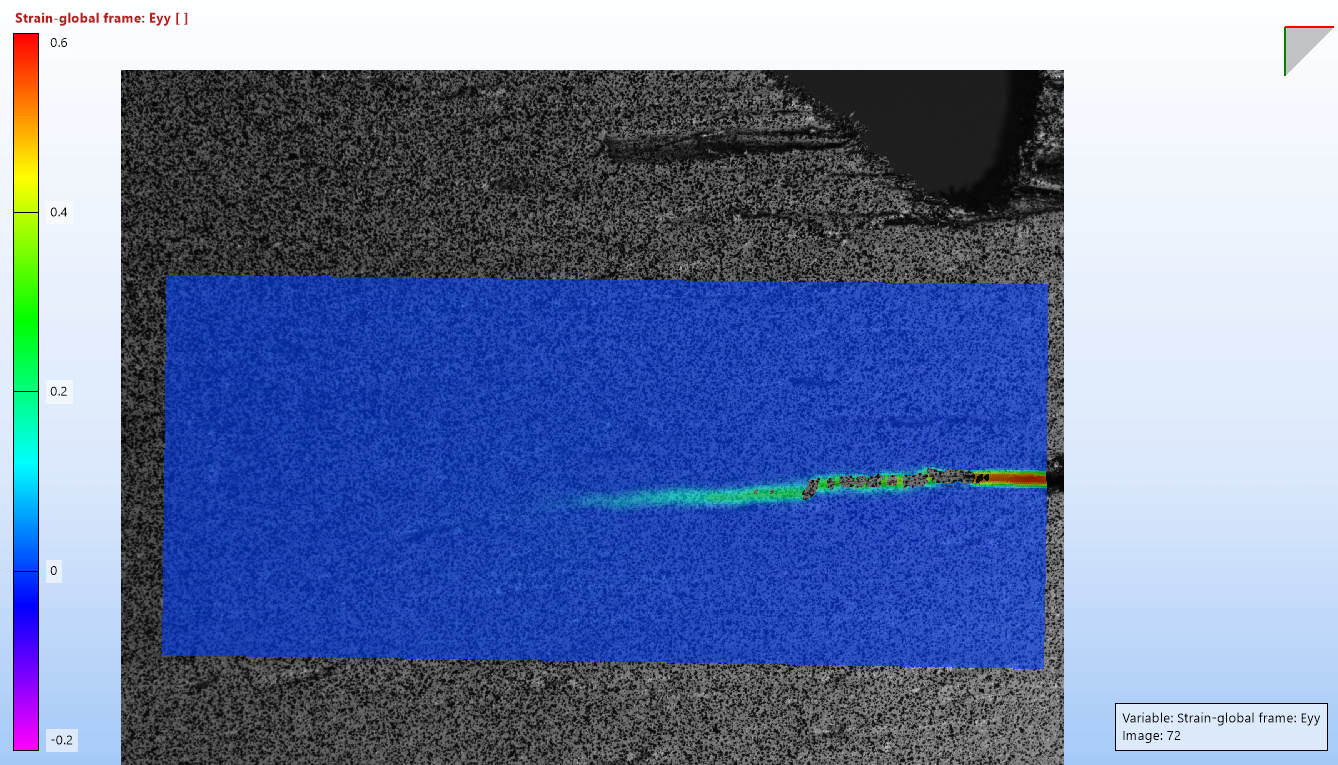
\includegraphics[width=9cm]{fig38}
	\caption{Example of deformation map specimen e2e2 ($\epsilon$yy)}
	\label{fig:fig38}
\end{figure}

Strain maps are used to best locate the position of the the crack tip by graphic reading.
Thus, thanks to the deformation maps we are able to obtain the crack length on different stages. It is then possible to check whether method 1 is working correctly.
The blue points figure \ref{fig:fig39} and \ref{fig:fig40} for tests e2e2 and e4e1 are the points read graphically with the deformation maps. It can be seen that the blue points follow the curve of method 1 correctly, so we can consider that method 1 works and that we can use it for all the tests.

\begin{figure}[htp]
	\begin{minipage}[c]{.46\linewidth}
		\centering
		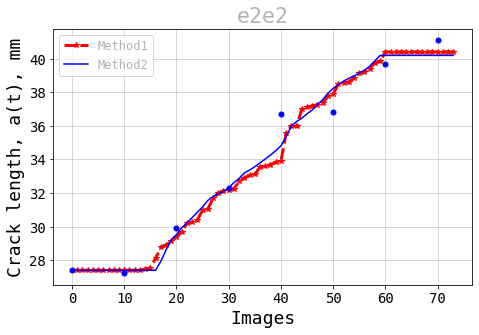
\includegraphics[width=7cm]{fig39}
		\caption{$\overline{VD}$ and $VD_{th}$ with Joao's data}
		\label{fig:fig39}
	\end{minipage}
	\hfill%
	\begin{minipage}[c]{.46\linewidth}
		\centering
		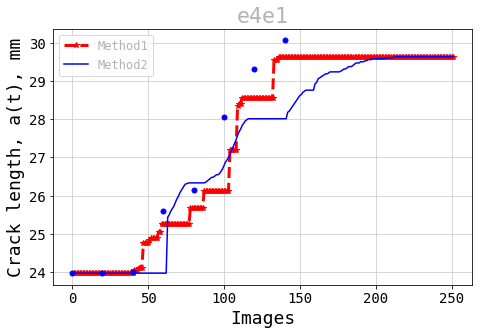
\includegraphics[width=7cm]{fig40}
		\caption{$\overline{VD}$ and $VD_{th}$ with MMCG data}
		\label{fig:fig40}
	\end{minipage}
\end{figure}


\section{Force - Crack opening curve}

The crack opening curves are presented in Figures x. It is obtained from the displacement maps and using the methodology presented in method 1.

Add some plots later

\section{Force-Crack length curve}

Figure x shows an example of the evolution of the force as a function of the crack length. The crack length increases gradually and continuously before rupture. It is the design of its shape that allows the stable propagation of the crack. Indeed, with this specimen, cracks progress slowly until failure occurs at maximum force.

\section{Critical energy restitution rate}

\section{Discussion}

Table \ref{fig:fig37} compares the different values obtained in this study with literature values obtained on temperate species. These are numerous, especially in mode I. In order to provide an objective comparison, the discussion focuses on temperate species with the same density and an initial crack oriented in the RL direction.


\begin{table} \centering
	\begin{tabular}{ccccccc}
		\toprule % horizontal line at the top of the table
		& References & Wood species & Test type & Orientation & Density & $G_{max}(J/m^2)$\\\midrule
		& \cite{Mambili2018} & Normal poplar & 2MCG & RL & 0.35-0.5 & 1287\\\midrule
		& \cite{Mambili2018} & Tension poplar & 2MCG & RL & 0.35-0.5 & 430\\\midrule
		& \cite{Mambili2018} & Normal white fir & 2MCG & RL & 0.53 & 761\\\midrule
		& \cite{Mambili2018} & Compression white fir & 2MCG & RL  & 0.53 & 1169\\\midrule
		& \cite{Odounga2018phd} & Okoumé & 2MCG & RL & 0.39-0.5 & 317\\\midrule
		& \cite{Odounga2018phd} & Iroko & 2MCG & RL & 0.56-0.7 & 323\\\midrule
		& \cite{Odounga2018phd} & Padouk & 2MCG & RL & 0.7-0.88 & 255\\\midrule
		& \cite{Odounga2018phd} & Iroko & 2MCG & RL & 0.56-0.7 & 323\\\midrule
		& \cite{Reiterer2002} & Spruce & WS & RL & 0.479 & 323\\\midrule
		& \cite{Reiterer2002} & Alder & WS & RL & 0.553 & 255\\\midrule
		& \cite{Reiterer2002} & Oak & WS & RL & 0.553 & 348\\\midrule
		& \cite{Reiterer2002} & Ash & WS & RL & 0.701 & 551\\
		\bottomrule % horizontal line at the bottom of the table
	\end{tabular}
	\caption{Comparison of mean max G values for specimens in the literature}
	\label{fig:fig37}
\end{table}

\section{Conclusion}